
This course has been tested on NIS Elements version 5.42.

\subsection{General interface}


\paragraph{Preliminary steps}
Once the GA3 module opened, other windows cannot be opened, therefore
\begin{itemize}
    \item you will need to open the image you want to work with first,
    \item it is convenient to open the LUT tools first (\keys{\ctrl+\Alt+L}),
    \item opening the help  can also be useful.
\end{itemize}
To access the GA3 interface, you can either:
\begin{itemize}
    \item use the menu \menu{Image>New GA3 recipe\dots},
    \item use the menu \menu{Image>Analysis Explorer\dots} to open the analysis exporter and then click on \menu{Create New},
    \item right-click on the background of the interface, select \menu{Analysis Controls>Analysis Explorer} to open the analysis explorer and then click on \menu{Create New}.
\end{itemize}

\paragraph{Loading and saving recipes}

\begin{itemize}
    \item Use \menu{Save} or \menu{Save As} to save the recipe in the local database. It will be then listed in the Analysis Explorer.
    \item Use your name as a prefix so that we can contact you if the database needs to be cleared.
    \item Use \menu{Export} to export the recipe in a folder of your choice. This recipe can then be reloaded on another computer. It is good practice to have a copy of the recipes in that way.
    \item Use \menu{Import} to reload an exported recipe. 
\end{itemize}

\paragraph{Recipes}
\begin{figure*}
    \centering \small
    \begin{tikzpicture}
        \node at (0,0) {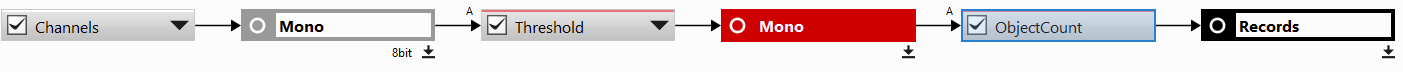
\includegraphics[width=0.75\textwidth]{artwork/simple-workflow.png}};
        % \draw[gray,very thin,step=1] (-5,-1) grid (5,1);
        \node (a) at (-5,-0.5){color};
        \node (b) at (-2.5,-0.5) {action};
        \node (c) at (0,-0.5) {binary};
        \node (d) at (5,-0.5) {table};
        \draw[->] (a) -| ++(1,0.4); 
        \draw[->] (b) -| ++(1,0.4); 
        \draw[->] (c) -| ++(1,0.4); 
        \draw[->] (d) -| ++(1,0.4); 
    \end{tikzpicture}
    \caption{A simple workflow with three kinds of nodes.}
    \label{fig:nodes}
\end{figure*}

Recipes describe a workflow as a graph. The graph is composed of 4 types of nodes (See Fig.~\ref{fig:nodes}):
\begin{enumerate}\setlength\itemsep{0em}
    \item color: original or processed grayscale images
    \item action: processing steps on images, binary or tables
    \item binary: masks and labels
    \item results: tables with measurement results 
\end{enumerate}

To add an action, drag the new element to the previous one to automatically create a connection and keep the elements organized. You can also use \keys{\shift} and left click circling the elements to select them. Finally, a group of elements can be combined to create a function.

\paragraph{Storing results}

Saving of channels and binary layers can be enabled case by case using a right click on the layer and selecting ``store this result'' or ``do not store this result''.


\subsection{Tips}
\begin{itemize}
    \item Use \keys{\Alt+\arrowkeyup} / \keys{\Alt+\arrowkeydown}  to increase / decrease the opacity of the binaries.
    \item To look for a module, use the search bar at the top.
    \item Right-click on the image and find image information for pixel to micron conversion.
    \item Click on the question mark on each operation (top left) for more information if needed.
\end{itemize}

\subsection{Basic image processing concepts}

\paragraph{Image} An image is any array (table) of regularly sampled intensity value. The values can range between $0$ and $2^8 = 255$ for 8-bit images or between $0$ and $2^{16}=65635$ for 16 bit images. Figure~\ref{fig:median} displays an image as graylevel and intensities values.

\paragraph{Threshold} Threshold is the simplest form of image segmentation. At each location of the image, a decision is taken to classify this point as foreground or background. In GA3, thresholds are followed by other operations such as smoothing, cleaning, connected component labelling, size filtering,\dots Here threshold are defined by a range with a minimum and maximum intensity. In fluorescence microscopy, we often want the minimum of this range to be more than 0 and the maximum untouched.

\paragraph{Median filter} The median filter is creating a new image where each pixel is computed as the median value of the pixels in a neighborhood of this pixel (See Figure~\ref{fig:median}). The median filter is a good approach for reducing the noise whilst preserving the edges of the image.

\begin{figure}[ht]\centering
    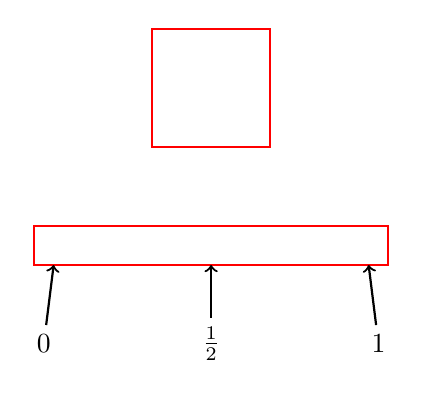
\begin{tikzpicture}[scale=0.5]
    \begin{scope}
        \def\pixels{{10,5,6,2,9},{8,5,2,4,8},{4,8,6,3,1},{2,9,7,10,3},{3,6,6,2,9}}
        \showpixelsvalue{\pixels}{0}{10}
        \draw[red,thick] (2,2) rectangle +(3,3);
    \end{scope}
    \begin{scope}[yshift=-2cm,xshift=-2cm]
        \def\pixels{{2,3,4,5,6,7,8,9,10}} 
        \showpixelsvalue{\pixels}{0}{10}
        \draw[red,thick] (1,1) rectangle +(9,1);
        \draw (1.25,-1) node {$0$} edge[->,thick] (1.5,1);
        \draw (5.5,-1) node {$\frac{1}{2}$} edge[->,thick] (5.5,1);
        \draw (9.75,-1) node {$1$} edge[->,thick] (9.5,1);
    \end{scope}
    \end{tikzpicture}
    \caption{Values in a $3 \times 3$ neighborhood are ordered to define a median (rank 1/2)
    filter. The intensity corresponding to the median value is stored in a new image.}
    \label{fig:median}
\end{figure}

\paragraph{Morphological erosion and dilation} Erosion and dilation are morphological operations on the image. They can be expressed both for binary and grayscale images are the minimum and respectively maximum of the pixels in a neighborhood depicted in red in Figure.~\ref{fig:median}, \textit{i.e.} ranks 0 and 1. In practice, this neighborhood could have various shapes and also have a different weight. Formally, the erosion of a and image $f$ at each pixel $x$ by a structuring element with weights $b$ defined as $(f \oplus b)(x) = \inf_{y} f(x+y) - b(y)$ and the dilation as $(f \ominus b)(x) = \sup_{y} f(y) + b(x-y)$. The result is an image with smaller, and respectively bigger, bright areas enabling to expand and shrink region.

\paragraph{Morphological opening and closing} Opening and closing are also morphological operations resulting of the combination an erosion followed by a dilation, and respectively, the dilation followed by an erosion. Formally, the opening is defined as $f \circ b  = (f \ominus b) \oplus b$ and the closing is defined as $f \bullet  b  = (f \oplus b) \ominus b$.

\paragraph{Rolling ball} Rolling ball~\cite{sternberg1983} is used for correcting shading and non-even background. It works by subtracting a background image estimated by a morphological opening the image using a structuring element which has radially decaying weights (the ball).

\begin{figure}[ht]\centering
    \begin{tikzpicture}[scale=0.8]
        \begin{axis}[
            axis lines=left, 
            xlabel={$x$},
            ylabel={gray levels},
            domain=0:10,
            grid=major,
            samples=200,
            ymin=0.25,
        ]
        \draw [gray,fill,opacity=0.5] (3.4,0.6) ellipse [x radius=1.35, y radius=0.25]; 
        \node (c) at (7,0.6){Rolling ball};
        \addplot[plum1,very thick] {exp(-(x-8)^2 / 100)};
        \addplot[red,very thick] {0.8*exp(-(x-3)^2 / 0.2)+exp(-(x-7)^2 / 0.25)+exp(-(x-8)^2 / 100)};
        \addplot[chameleon1,very thick] {0.055*exp(-(x-3)^2 / 0.4)+0.05*exp(-(x-7)^2 / 0.4)+exp(-(x-8)^2 / 100)};
        \draw[->] (c) -- (5,0.6);
        \end{axis} 
    \end{tikzpicture}
    \caption{Illustration of the rolling ball.}
    \label{fig:algorithm}
\end{figure}

\begin{figure}[ht]\centering
    \begin{tikzpicture}[scale=0.8]
        \begin{axis}[
            axis lines=left, 
            xlabel={$x$},
            ylabel={gray levels},
            domain=0:10,
            grid=major,
            samples=200,
            ymin=0.0,
            ymax=1.2,
        ]
        \addplot[red,very thick,name path=A] {1-(0.7*exp(-(x-2.5)^2 / 0.3)+0.9*exp(-(x-5)^2 / 0.25)+0.6*exp(-(x-8)^2 / 0.5))-0.1*exp(-(x-8)^2 / 80)};
        \addplot+[draw=none, no markers, name path=B] {1}; 
        \addplot[skyblue1,opacity=0.7] fill between[
            of=A and B,
            soft clip={domain=0:3.8}
        ];
        \addplot[plum1,opacity=0.7] fill between[
            of=A and B,
            soft clip={domain=3.8:6.2}
        ];        
        \addplot[chameleon1,opacity=0.7] fill between[
            of=A and B,
            soft clip={domain=6.2:10}
        ];
        
        \end{axis} 
    \end{tikzpicture}
    \caption{Illustration of the watershed algorithms of the digital elevation model (DEM) with 3 flooded depressions. The seeds or sources are the local minima of the DEM.}
    \label{fig:watershed}
\end{figure}



\paragraph{Watershed} The watershed algorithm associate to seed regions pixels in the image in the order of a priority map. It can also be interpreted as flooding a landscape or digital elevation model (DEM) (see Figure~\ref{fig:watershed}). In practice, several algorithms can be considered for implementing a watershed. One of them is called ``priority-flood''~\cite{barnes2014} where starting from seeds, each neighboring pixels (e.g. $3 \times 3$) are added to a queue by order of priority given by a priority map (minimum elevation of the landscape). The queue keeps track of the priority value, the location and the label of the basin. Seeds can be defined as local minima of the landscape function. At each iteration, the highest priority element is popped out of the queue, if not already labeled the pixel if attributed the label of the current basin and its neighbors added to the queue.

\paragraph{Pearson correlation coefficient} The Pearson correlation coefficient (PCC)~\cite{pcc} is a statistical tool used to measure the linear correlation between two signal indicating the potential co-localization of two labelled molecules population. If we have the pair of red and green intensities $(r_i,g_i)$ at each location $i$ in the image, the PCC is defined as 
$$\mathrm{pcc} = \frac{\sum_i(r_i-\bar{r})(g_i-\bar{g})}{\sum_i(r_i-\bar{r})^2 \sum_i(g_i-\bar{g})^2}$$ 
with the means $\bar{r} = n^{-1}\sum_i r_i$ and $\bar{g} = n^{-1}\sum_i g_i$. The value of the PCC ranges from -1 to 1 where a value of 1 indicates a linear correlation.

\paragraph{Table join} To combine measurements from two tables, we can use a ``join''~\cite{join} which will find the  rows base sharing a common reference index. The ``inner join'' operation will include only the matching row in both tables (See Figure~\ref{fig:join}). Manipulating table can replace logical operation on binary masks when combined with object parenting. In the simpler case where table have the same corresponding rows in the same order, tables can be simply collated with each other.

\begin{figure}[ht]\centering
    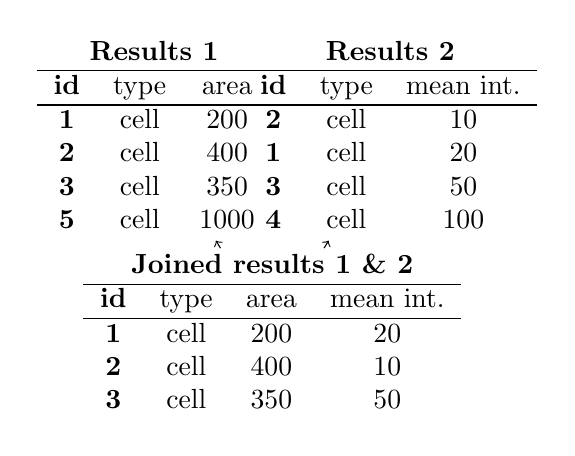
\begin{tikzpicture}
        \node (A) at (0,2.5) {
            \begin{tabular}{>{\bfseries}ccc}
                \multicolumn{3}{c}{\textbf{Results 1}}\\ \hline
                id & type & area \\ \hline
                1  & cell & 200 \\
                2  & cell & 400 \\
                3  & cell & 350  \\
                5 & cell & 1000 
            \end{tabular}
        };
        \node (B) at (3,2.5) {
            \begin{tabular}{>{\bfseries}ccc}
                \multicolumn{3}{c}{\textbf{Results 2}}\\ \hline
                id & type & mean int. \\ \hline
                2  & cell & 10 \\
                1  & cell & 20 \\
                3  & cell & 50 \\
                4  & cell & 100 
            \end{tabular}
        };
        \node (C) at (1.5,0) {
            \begin{tabular}{>{\bfseries}cccc}
                \multicolumn{4}{c}{\textbf{Joined results 1 \& 2}}\\ \hline
                id & type & area & mean int.\\ \hline
                1  & cell & 200 & 20\\
                2  & cell & 400 & 10\\
                3  & cell & 350 & 50
            \end{tabular}
        };
        \draw[->] (A)--(C);
        \draw[->] (B)--(C);
        \end{tikzpicture}
\caption{Inner join of two tables based on the column id.}
\label{fig:join}
\end{figure}



\subsection{Sample preparation and microscopy}

Lots of time can be saved by adjusting sample preparation and imaging to match existing  analysis tools.

\paragraph{Housekeeping labels} If possible, and when aiming at cell level statistics, include extra labels that will help identify cells location during sample preparation. A DNA stains such as DAPI and Hoescht and a plasma membrane marker such as WGA, Invitrogen's CellMask or Biotium's CellBrite can be used for example. 

\paragraph{Cell confluence} Depending on the type of analysis workflow and the cell line, high cell confluence can be counterproductive as cell will tend to grow on top of each other.

\paragraph{Dataset size} When acquiring data, have in mind the scale of the process you want to capture. If only a fraction of the cells are of interest, define multiple position instead of tiling a large field of view at high resolution will reduce the size of the dataset.





